\section{收敛与计算成本}
\label{sec:tr-convergence}

前几节的例子看起来都收敛了，在什么条件下这是必然的，极限点是什么样的点，每一轮又要花多少计算？

\paragraph{假设}
一阶结果需要下面三条假设。
\begin{enumerate}
 \item $f$连续可微，下有界，$f\geq f_{\mathrm{low}}$，梯度在$\mathbb{R}^n$上Lipschitz连续，常数为$L$。
 \item 模型矩阵一致有界：$\bm{B}^{(t)}$对称，$\lVert\bm{B}^{(t)}\rVert_2\leq M$，$M>0$。
 \item 候选步可行，$\lVert\bm{p}^{(t)}\rVert_2\leq\Delta^{(t)}$，并且对某个$c_1\in(0,1]$满足充分模型下降：
 \begin{equation}
  \operatorname{pred}(\bm{p}^{(t)})\geq c_1\lVert\bm{g}^{(t)}\rVert_2\min\Bigl\{\Delta^{(t)},\ \frac{\lVert\bm{g}^{(t)}\rVert_2}{M}\Bigr\}.
  \label{eq:tr-assumption-decrease}
 \end{equation}
\end{enumerate}

第三条由式~\eqref{eq:tr-sufficient-decrease}和$\lVert\bm{B}^{(t)}\rVert_2\leq M$推出，前面三种求解器都满足。第一条的全局Lipschitz条件可以放宽：目标~\eqref{eq:tr-example}的梯度不是全局Lipschitz的，但它的水平集有界，半径又有上限$\Delta_{\max}$，试探点都落在一个紧集内，$L$只需在这个紧集上成立。

条件里没有要求$\bm{B}^{(t)}$接近Hessian，也没有要求子问题解得精确。模型只要在一阶上与目标匹配，这正是拟牛顿模型能够进入这个框架的原因。

\paragraph{半径不会塌缩}
证明的核心是一个观察：半径足够小时，模型误差相对预测下降可以忽略，这一步一定被接受。模型误差是半径的二次量，预测下降却是半径的一次量，两者之比随半径趋于零。图~\ref{fig:tr-radius-rho}在点$\bm{a}$上验证了这一点：取精确Hessian时$\lvert1-\rho\rvert$随半径的斜率是$2$，取粗糙的$\bm{B}=\bm{I}$时斜率是$1$，后者正是定理使用的一般界。

\begin{BookInlineFigure}
 \centering
 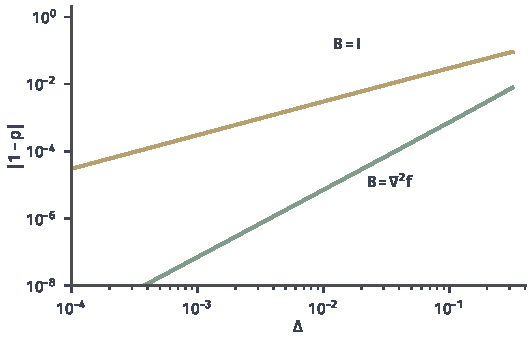
\includegraphics[width=90mm]{figures/05-optimization/02-smooth-optimization/matplotlib/tr-radius-rho/figure.pdf}
 \caption{在点$\bm{a}$沿负梯度方向取长度$\Delta$的步，$\lvert1-\rho\rvert$随$\Delta$的变化（对数坐标）。绿线的模型矩阵是Hessian，斜率约为$2$；黄线的模型矩阵是$\bm{I}$，斜率约为$1$。两条线都随$\Delta\to0$趋于零。}
 \label{fig:tr-radius-rho}
\end{BookInlineFigure}

\begin{theorem}[梯度的下极限为零]
 \label{thm:tr-first-order}
 在上述三条假设下，设外层迭代按式~\eqref{eq:tr-accept}和式~\eqref{eq:tr-radius}更新，其中$\eta_1>0$。此时
 \begin{equation}
  \liminf_{t\to\infty}\lVert\bm{g}^{(t)}\rVert_2=0.
  \label{eq:tr-liminf}
 \end{equation}
\end{theorem}

\begin{proof}
 反设存在$\varepsilon>0$和$T_0$，使得$t\geq T_0$时$\lVert\bm{g}^{(t)}\rVert_2\geq\varepsilon$。

 第一步估计模型误差。由梯度Lipschitz连续，对任意$\bm{p}$，
 \[
  \bigl\lvert f(\bm{x}+\bm{p})-f(\bm{x})-\langle\bm{g},\bm{p}\rangle\bigr\rvert
  =\Bigl\lvert\int_0^1\langle\nabla f(\bm{x}+s\bm{p})-\bm{g},\bm{p}\rangle\,\mathrm{d}s\Bigr\rvert
  \leq\frac{L}{2}\lVert\bm{p}\rVert_2^2.
 \]
 再计入模型的二次项，且$\lVert\bm{p}^{(t)}\rVert_2\leq\Delta^{(t)}$，得到
 \[
  \bigl\lvert f(\bm{x}^{(t)}+\bm{p}^{(t)})-m^{(t)}(\bm{p}^{(t)})\bigr\rvert\leq\frac{L+M}{2}(\Delta^{(t)})^2.
 \]

 第二步说明小半径时不会缩小。令
 \[
  K=\min\Bigl\{\frac1M,\ \frac{2c_1(1-\eta_2)}{L+M}\Bigr\}.
 \]
 设$t\geq T_0$且$\Delta^{(t)}\leq K\varepsilon$。此时$\Delta^{(t)}\leq\varepsilon/M$，不超过$\lVert\bm{g}^{(t)}\rVert_2/M$，所以式~\eqref{eq:tr-assumption-decrease}的最小值取在$\Delta^{(t)}$上：
 \[
  \operatorname{pred}(\bm{p}^{(t)})\geq c_1\varepsilon\Delta^{(t)}.
 \]
 又$m^{(t)}(\bm{0})=f(\bm{x}^{(t)})$，所以预测下降与实际下降之差就是模型误差，于是
 \[
  \lvert1-\rho^{(t)}\rvert\leq\frac{(L+M)(\Delta^{(t)})^2/2}{c_1\varepsilon\Delta^{(t)}}=\frac{(L+M)\Delta^{(t)}}{2c_1\varepsilon}\leq1-\eta_2.
 \]
 因此$\rho^{(t)}\geq\eta_2\geq\eta_1$，这一轮半径不缩小。

 第三步得到半径的下界。半径只在$\Delta^{(t)}>K\varepsilon$时才可能缩小，缩小后不低于$\theta K\varepsilon$，所以对$t\geq T_0$，
 \[
  \Delta^{(t)}\geq\Delta_{\min}:=\min\{\Delta^{(T_0)},\ \theta K\varepsilon\}>0.
 \]

 第四步导出矛盾。若被接受的轮只有有限多次，则此后点不动，半径每轮乘以$\theta$，趋于零，与下界矛盾。所以接受无穷多次，每次接受时$\rho^{(t)}\geq\eta_1$，并由式~\eqref{eq:tr-assumption-decrease}，
 \[
  f(\bm{x}^{(t)})-f(\bm{x}^{(t+1)})\geq\eta_1\operatorname{pred}(\bm{p}^{(t)})
  \geq\eta_1c_1\varepsilon\min\Bigl\{\Delta_{\min},\ \frac{\varepsilon}{M}\Bigr\}>0.
 \]
 目标值单调不增，却无穷多次下降一个固定的量，这与$f\geq f_{\mathrm{low}}$矛盾。
\end{proof}

下极限只说明有一个子列的梯度趋于零。$\eta_1>0$时可以加强：整个序列的梯度都趋于零。

\begin{theorem}[梯度趋于零]
 \label{thm:tr-limit}
 在定理~\ref{thm:tr-first-order}的条件下，
 \begin{equation}
  \lim_{t\to\infty}\lVert\bm{g}^{(t)}\rVert_2=0.
  \label{eq:tr-limit}
 \end{equation}
\end{theorem}

\begin{proof}
 反设存在$\varepsilon>0$和无穷多个下标$t$满足$\lVert\bm{g}^{(t)}\rVert_2\geq2\varepsilon$。对每个这样的$t$，由定理~\ref{thm:tr-first-order}，存在最小的$l(t)>t$使$\lVert\bm{g}^{(l(t))}\rVert_2<\varepsilon$。在$t\leq k<l(t)$的轮中$\lVert\bm{g}^{(k)}\rVert_2\geq\varepsilon$。记其中被接受的轮的集合为$\mathcal{K}$。

 由Lipschitz条件和$\lVert\bm{p}^{(k)}\rVert_2\leq\Delta^{(k)}$，这段路程的总长度不能太短：
 \[
  \varepsilon\leq\lVert\bm{g}^{(t)}\rVert_2-\lVert\bm{g}^{(l(t))}\rVert_2\leq L\sum_{k\in\mathcal{K}}\lVert\bm{p}^{(k)}\rVert_2\leq L\sum_{k\in\mathcal{K}}\Delta^{(k)}.
 \]

 这段路程上目标的下降量由接受规则和式~\eqref{eq:tr-assumption-decrease}控制：
 \[
  f(\bm{x}^{(t)})-f(\bm{x}^{(l(t))})\geq\eta_1c_1\varepsilon\sum_{k\in\mathcal{K}}\min\Bigl\{\Delta^{(k)},\ \frac{\varepsilon}{M}\Bigr\}.
 \]

 若$\mathcal{K}$中某一项有$\Delta^{(k)}>\varepsilon/M$，右端至少是$\eta_1c_1\varepsilon^2/M$。否则右端等于$\eta_1c_1\varepsilon\sum\Delta^{(k)}$，至少是$\eta_1c_1\varepsilon^2/L$。两种情形下降量都有一个不依赖$t$的正下界。但$f(\bm{x}^{(t)})$单调且有下界，$t\to\infty$时$f(\bm{x}^{(t)})-f(\bm{x}^{(l(t))})\to0$，矛盾。
\end{proof}

条件的作用可以逐条核对。去掉下有界，目标可以一直下降，例如$f(x)=-x$，梯度恒为$-1$。去掉$\eta_1>0$的接受门槛，只要求$\rho^{(t)}>0$，下降量可以任意小，一般只能得到下极限的结论。去掉充分模型下降，候选步可以小到没有进展，比值$\rho^{(t)}$即使接近$1$也无济于事。

\paragraph{二阶保证}
定理~\ref{thm:tr-limit}只说明极限点是驻点，鞍点也是驻点。要排除负曲率，候选步必须真正使用负曲率。设$\bm{B}^{(t)}=\bm{H}^{(t)}$，用下面的量衡量负曲率的大小：
\[
 \lambda^{(t)}_-=\max\{0,\ -\lambda_{\min}(\bm{H}^{(t)})\}.
\]
要求存在常数$c_2>0$，使得
\begin{equation}
 \operatorname{pred}(\bm{p}^{(t)})\geq c_2\lambda^{(t)}_-(\Delta^{(t)})^2.
 \label{eq:tr-eigen-decrease}
\end{equation}

子问题的全局解满足这一条，$c_2=1/2$。取$\bm{u}$是$\lambda_{\min}$的单位特征向量，选符号使$\langle\bm{g},\bm{u}\rangle\leq0$，点$\Delta\bm{u}$可行，由它的模型值得
\[
 m(\bm{0})-m(\Delta\bm{u})=-\Delta\langle\bm{g},\bm{u}\rangle-\frac12\lambda_{\min}\Delta^2\geq\frac12\lambda_-\Delta^2,
\]
全局解的预测下降不低于这个量。

Cauchy步和截断共轭梯度不满足式~\eqref{eq:tr-eigen-decrease}。第~\ref{sec:tr-model}节困难情形的数据$\bm{g}=(0,1)^\top$，$\bm{B}=\operatorname{diag}(-1,3)$，$\Delta=1$就是反例。截断共轭梯度第一步$\bm{d}^{(0)}=(0,-1)^\top$，曲率为正，一步到$(0,-1/3)^\top$，残差为零而停止，预测下降只有$1/6$。全局解的预测下降是$5/8$，并且沿$\bm{e}_1$方向使用了负曲率。迭代只在Krylov子空间中进行，而这个子空间恰好与$\bm{e}_1$正交，图~\ref{fig:tr-second-order}(a)画出了这一点。若$\bm{g}=\bm{0}$，迭代第一步就停在$\bm{p}=\bm{0}$，负曲率完全看不到。

\begin{theorem}[二阶下极限]
 \label{thm:tr-second-order}
 在定理~\ref{thm:tr-first-order}的条件之外，设$\bm{B}^{(t)}=\bm{H}^{(t)}$，Hessian是$L_H$-Lipschitz的，且候选步满足式~\eqref{eq:tr-eigen-decrease}。则
 \begin{equation}
  \liminf_{t\to\infty}\max\bigl\{\lVert\bm{g}^{(t)}\rVert_2,\ \lambda^{(t)}_-\bigr\}=0.
  \label{eq:tr-second-order}
 \end{equation}
\end{theorem}

\begin{proof}
 反设存在$\varepsilon>0$和$T_0$，使得$t\geq T_0$时
 \[
  \max\{\lVert\bm{g}^{(t)}\rVert_2,\ \lambda^{(t)}_-\}\geq\varepsilon.
 \]
 若$\lVert\bm{g}^{(t)}\rVert_2\geq\varepsilon$，定理~\ref{thm:tr-first-order}证明的第二步依然适用。若$\lambda^{(t)}_-\geq\varepsilon$，由Hessian的Lipschitz条件，模型误差不超过$L_H\lVert\bm{p}\rVert_2^3/6$，再用式~\eqref{eq:tr-eigen-decrease}，
 \[
  \lvert1-\rho^{(t)}\rvert\leq\frac{L_H(\Delta^{(t)})^3/6}{c_2\varepsilon(\Delta^{(t)})^2}=\frac{L_H\Delta^{(t)}}{6c_2\varepsilon}.
 \]
 所以取$K_2=\min\{K,\ 6c_2(1-\eta_2)/L_H\}$，$\Delta^{(t)}\leq K_2\varepsilon$时半径不缩小，同样得到半径的正下界$\Delta_{\min}$。每次接受至少下降
 \[
  \eta_1\min\Bigl\{c_1\varepsilon\min\bigl\{\Delta_{\min},\ \varepsilon/M\bigr\},\ c_2\varepsilon\Delta_{\min}^2\Bigr\}>0,
 \]
 与定理~\ref{thm:tr-first-order}证明的第四步一样导出矛盾。
\end{proof}

这个定理给出的是一个子列上的结论：若该子列有极限点$\bar{\bm{x}}$，则$\nabla f(\bar{\bm{x}})=\bm{0}$且$\nabla^2f(\bar{\bm{x}})\succeq\bm{0}$。这只是二阶必要条件，并不说明$\bar{\bm{x}}$是局部极小点。图~\ref{fig:tr-second-order}(b)的$f(x)=x^3$在$x=0$处梯度和Hessian都为零，从这一点出发，任何候选步都不能使模型下降，算法立即停止，而这个点不是局部极小点。

$x^3$没有下界，这里只用它展示驻点附近的形状；把函数在远处改成有下界、导数Lipschitz的光滑函数，$x=0$附近的情形不变。

所以不能仅凭采用信赖域就声称找到了局部极小点，更谈不上全局最优。一阶保证只需要充分模型下降，二阶保证要求候选步真正利用负曲率，两者对子问题的精度要求不同。这种差别在第~\ref{chap:saddle-points}章有进一步的讨论。

\begin{BookInlineFigure}
 \centering
 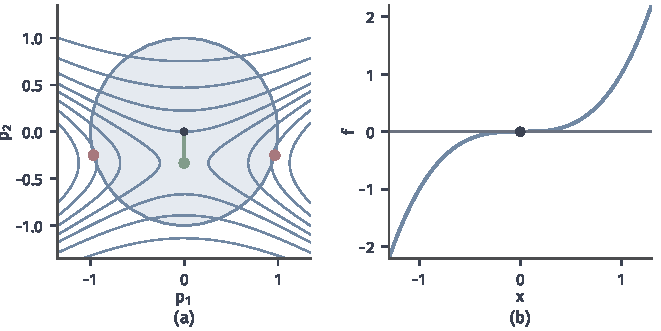
\includegraphics[width=112mm]{figures/05-optimization/02-smooth-optimization/matplotlib/tr-second-order/figure.pdf}
 \caption{二阶保证的两个边界。(a)~模型$\bm{g}=(0,1)^\top$，$\bm{B}=\operatorname{diag}(-1,3)$，$\Delta=1$：截断共轭梯度只沿$p_2$轴走到绿点，两个红点是全局解。(b)~$f(x)=x^3$，黑点处梯度和Hessian都为零，满足二阶必要条件，却不是局部极小点。}
 \label{fig:tr-second-order}
\end{BookInlineFigure}

\paragraph{迭代次数}
定理~\ref{thm:tr-first-order}的证明本身给出了复杂度。设前$T$轮都有$\lVert\bm{g}^{(t)}\rVert_2\geq\varepsilon$，半径有下界$\Delta_{\min}$，$\varepsilon$小时$\Delta_{\min}$与$\varepsilon$同阶。把第四步中每次接受的下降量代入总下降量$f(\bm{x}^{(0)})-f_{\mathrm{low}}$，可知接受的轮数$A$满足
\begin{equation}
 A\leq\frac{f(\bm{x}^{(0)})-f_{\mathrm{low}}}{\eta_1c_1\varepsilon\min\{\Delta_{\min},\ \varepsilon/M\}}=O(\varepsilon^{-2}).
 \label{eq:tr-accepted-count}
\end{equation}

拒绝的轮数$R$也受控制。半径每次接受至多乘以$2$，每次拒绝乘以$\theta$，且始终不低于$\Delta_{\min}$，所以$\Delta^{(0)}2^A\theta^R\geq\Delta_{\min}$，由此得到
\begin{equation}
 R\leq\frac{A\ln2+\ln(\Delta^{(0)}/\Delta_{\min})}{\ln(1/\theta)}.
 \label{eq:tr-rejected-count}
\end{equation}

因此外层总轮数是$O(\varepsilon^{-2})$，只比接受轮数多一个常数倍和一个对数项。这个阶与梯度下降相同，并且对信赖域Newton法也是紧的，构造最坏的目标需要专门设计的例子，篇幅较长，读者可查阅专门的优化复杂度文献。这也提醒我们，信赖域Newton法在实践中的优势来自局部收敛和对曲率的利用，不来自这个最坏情形的上界。

\paragraph{局部收敛}
设$\bm{x}^{(t)}\to\bm{x}^\star$，$\nabla^2f(\bm{x}^\star)\succ\bm{0}$，Hessian在$\bm{x}^\star$附近Lipschitz，并取$\bm{B}^{(t)}=\bm{H}^{(t)}$。靠近解时Newton步趋于零，比值$\rho^{(t)}$趋于$1$，半径不再缩小，Newton步终将落在球内。狗腿法、精确解都直接取Newton步，于是回到第~\ref{chap:second-order-methods}章的局部二次收敛。截断共轭梯度由残差停止，$\eta\to0$的快慢决定超线性或二次收敛，取$\eta=\min\{0.1,\sqrt{\lVert\bm{g}\rVert_2}\}$时是超线性的。表~\ref{tab:tr-history}中第$4$到第$7$轮就是这一阶段。这里只说明了机制，严格的证明还需要验证$\rho^{(t)}\to1$的速度，读者可查阅\scite{math-nocedal2006numerical}。

\paragraph{计算成本}
评价信赖域的成本要把外层和内层分开算，表~\ref{tab:tr-cost}按一次子问题列出。

\begin{BookInlineTable}
 \centering
 \begin{tabular}{lll}
  \toprule
  子问题解法 & 对$\bm{B}$的要求 & 一次求解的代价\\
  \midrule
  Cauchy步 & 对称 & $1$次矩阵向量乘积\\
  狗腿法 & 正定 & $1$次分解，约$n^3/3$\\
  截断共轭梯度 & 对称 & $j$次矩阵向量乘积，$j\leq n$\\
  精确解 & 对称 & 数次分解，约$n^3/3$每次\\
  \bottomrule
 \end{tabular}
 \caption{一次子问题的代价，稠密矩阵，只计主要运算。}
 \label{tab:tr-cost}
\end{BookInlineTable}

外层每一轮需要一次函数值$f(\bm{x}^{(t)}+\bm{p}^{(t)})$；只有被接受的轮才需要新的梯度和$\bm{B}$，拒绝的轮只多一次子问题和一次函数值。Hessian向量乘积不必形成整个矩阵，用梯度差近似时，一次乘积大约是一次梯度的代价：
\begin{equation}
 \bm{H}^{(t)}\bm{v}\approx\frac{\nabla f(\bm{x}^{(t)}+h\bm{v})-\nabla f(\bm{x}^{(t)})}{h}.
 \label{eq:tr-hessian-vector}
\end{equation}
所以比较方法时不能只看外层轮数，要把内层的乘积次数也算进去。拒绝也不是免费的：当函数值很贵时，半径初值和更新因子要避免频繁试探。

图~\ref{fig:tr-methods-compare}是一个$n=20$的实验，目标是
\[
 f(\bm{x})=\sum_{i=1}^{19}\bigl[10(x_{i+1}-x_i^2)^2+(1-x_i)^2\bigr].
\]
三种方法的外层框架相同，参数同前。精确Hessian配截断共轭梯度用$26$个外层轮次、$157$次Hessian向量乘积把梯度降到$10^{-7}$以下。SR1模型从$20\bm{I}$出发，用$90$轮，每轮要多算一次梯度，但完全不用Hessian。只用Cauchy步时，$1200$轮后梯度仍有$1.8\times10^{-4}$。三者都满足第~\ref{sec:tr-convergence}节开头的假设，收敛定理对它们一视同仁，实际差距来自模型和子问题利用了多少曲率。

\begin{BookInlineFigure}
 \centering
 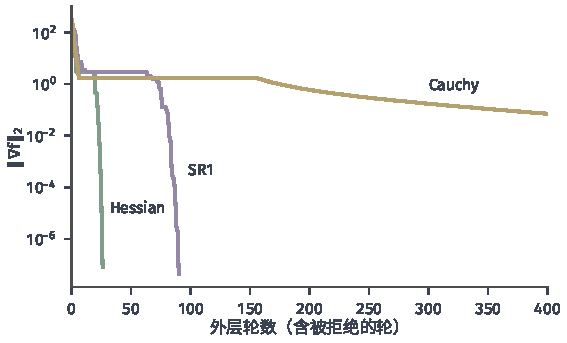
\includegraphics[width=96mm]{figures/05-optimization/02-smooth-optimization/matplotlib/tr-methods-compare/figure.pdf}
 \caption{同一信赖域框架下三种选择的梯度范数（到当前轮为止的最小值，对数坐标）。绿线是Hessian配截断共轭梯度，紫线是SR1模型配截断共轭梯度，黄线是Hessian配Cauchy步。横轴的轮数包含被拒绝的轮。目标是正文中的$20$维函数，每个奇数位分量初值为$-1.2$，其余为$1$。}
 \label{fig:tr-methods-compare}
\end{BookInlineFigure}
